\mode*


\section{Grannmatriser och -listor}

\begin{frame}
  \begin{columns}[b]
    \begin{column}{0.5\columnwidth}
      \begin{table}
        \begin{tabular}{rrrrrrr}
            & A & B & C & D & E & F \\
          A &   & 8 & 5 & 6 &   &   \\
          B &   &   & 2 &   &   &   \\
          C &   &   &   & 3 &   &   \\
          D &   &   &   &   & 1 &   \\
          E & 4 &   &   &   &   &   \\
          F &   &   &   &   &   &
        \end{tabular}
        \caption{Grannmatris}
      \end{table}
    \end{column}
    \begin{column}{0.5\columnwidth}
      \only<2>{
        \begin{figure}
          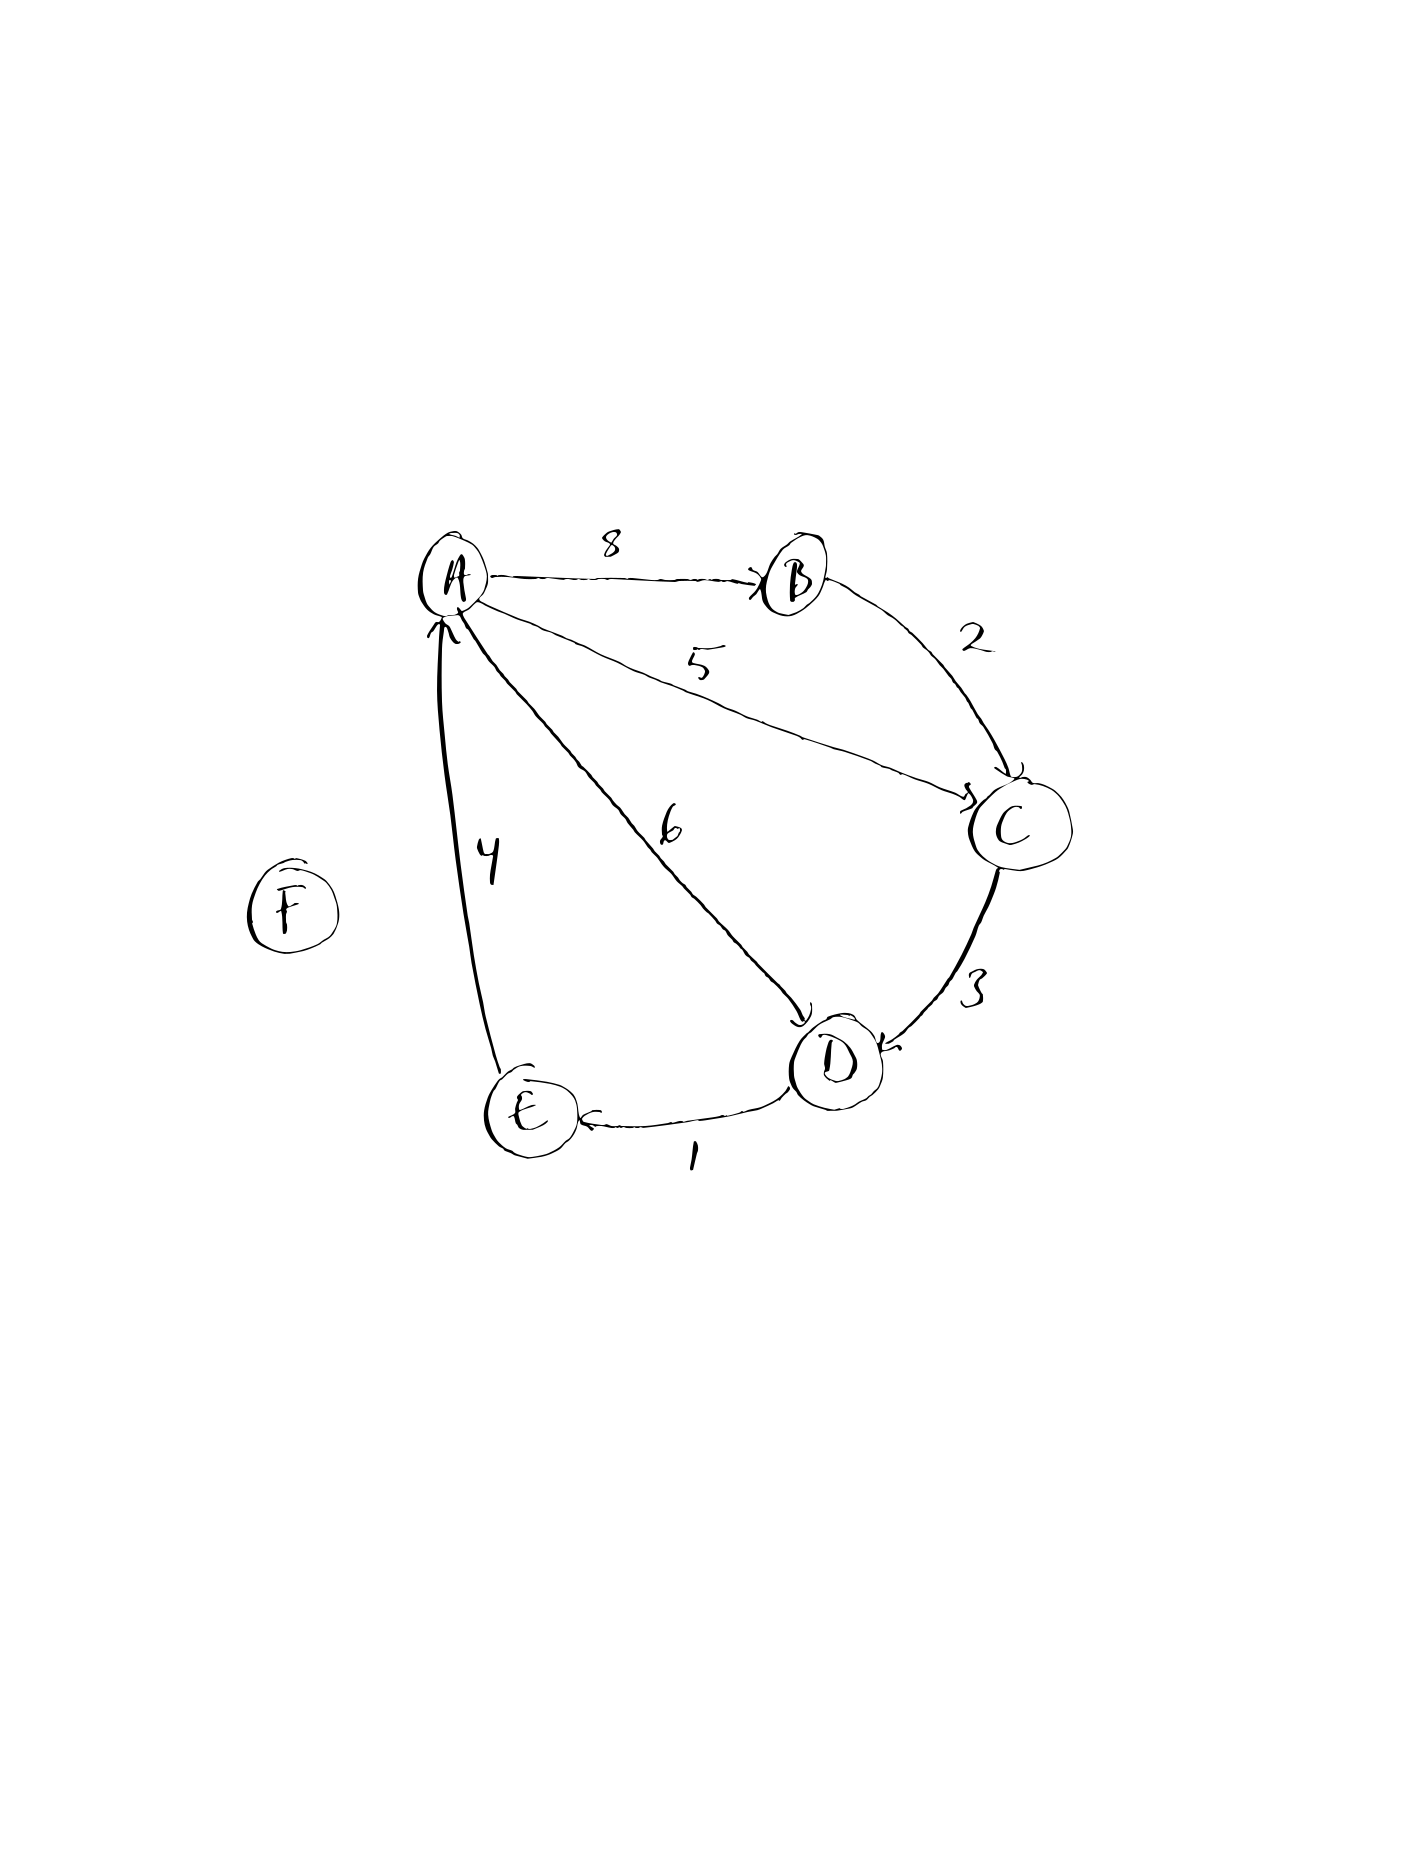
\includegraphics[width=\columnwidth]{fig/graph.pdf}
          \caption{Graf}
        \end{figure}
      }
    \end{column}
  \end{columns}
  \begin{exercise}
    \begin{itemize}
      \item Rita upp den graf som grannmatrisen ovan representerar.
      \item Skriv också upp motsvarande grannlistor.
      \item Vilken representation är mest sparsam?
    \end{itemize}
  \end{exercise}
\end{frame}


\section{Långa strykord}

\begin{frame}
  \begin{exercise}
    \begin{itemize}
      \item Ordet orkan är ett strykord eftersom man kan stryka sista bokstaven 
        om och om igen och bara få riktiga ord.
      \item orkan - orka - ork - or - o
      \item Uppgiften är att finna det längsta strykordet i svenska språket.
    \end{itemize}
    \begin{enumerate}
      \item Rita problemträdet och jämför olika tänkbara algoritmer.
      \item Skriv pythonkoden.
    \end{enumerate}
  \end{exercise}
\end{frame}

\begin{frame}
  \begin{solution}[Strykord]
    \inputminted[firstline=3,lastline=13]{python}{src/strykord.py}
  \end{solution}
\end{frame}

\begin{frame}
  \begin{solution}[Strykord fortsättning]
    \inputminted[firstline=15,lastline=23]{python}{src/strykord.py}
  \end{solution}
\end{frame}


\section{Skriva 100 med sjuor}

\begin{frame}
  \begin{exercise}
    \begin{itemize}
      \item Det gäller att skriva talet 100 med enbart sjuor och dom fyra 
        räknesätten, till exempel så här.
      \item \(7 + 7 / 7 \cdot 7 \cdot 7 = 98\)
      \item Det var ett gott försök som inte nådde ända fram.
      \item För att man ska få använda / måste divisionen gå jämnt ut.
    \end{itemize}
    \begin{enumerate}
      \item Rita problemträdet och diskutera bästa algoritm för att avgöra OM 
        problemet är lösbart.
      \item Om man dessutom vill veta hur lösningen ser ut krävs en mer 
        komplicerad datastruktur.
        Beskriv den och skissa ett program.
    \end{enumerate}
  \end{exercise}
\end{frame}

\begin{frame}
  \begin{solution}[Sjuor]
    \inputminted[firstline=17,lastline=25]{python}{src/sjuor.py}
  \end{solution}
\end{frame}

\begin{frame}
  \begin{solution}[Sjuor fortsättning]
    \inputminted[firstline=3,lastline=15]{python}{src/sjuor.py}
  \end{solution}
\end{frame}
